\chapter{Asking Millionaires How They Got Rich! (New York City)}

We are not given a single unified doctrine of wealth at the outset. Instead, the lecture proceeds by repeated questioning across a sequence of cases. The cold open promises the scale of the inquiry: \(\$22\) million years, harsh rules, low starting points, and celebrity testimony. The body of the lecture then slows down and asks, again and again: what was the scale, what was the turning point, what rule mattered, and what can be transferred? Read in that order, the chapter has a clear mathematical spine. It is built from cash floors, surplus, compounding horizons, return targets, sales volume, and the distinction between visible status and actual economic fit.

\section{New York as a Field Laboratory}

The lecture begins with a preview reel. We are shown fragments of real estate, finance, discipline, and large annual totals before the host states the governing premise: New York City is the city with the most millionaires, and it will therefore be used as a field site. That framing matters. The chapter should not read as a bag of isolated quotations. It should read as a controlled sequence of comparisons carried out in a dense economic environment.

The host's method is almost algorithmic. From one speaker to the next, the same prompts return:
\begin{itemize}
\item How much did you make?
\item What was the turning point?
\item What rule or lesson mattered?
\item What does this imply for somebody starting now?
\end{itemize}
The lecture is therefore cumulative. Each interview adds a new variable to the same larger problem.

\section{Wall Street as Selection Pressure}

The first complete case concerns finance. Characteristically, the lecture begins not with biography but with scale: the speaker's best month was about
\begin{equation}
Y_{\text{best month}} \approx \$80{,}000.
\end{equation}
But the point of the interview is not to leave that number standing by itself. Immediately we are told that Wall Street is a beast, savage, and full of rapid attrition. The speaker asks us, in effect, to look sideways and see how few people remain. Large inflow and high failure rate are presented together.

That pairing is the first important move of the lecture. Wealth is not introduced as a static total. It is introduced as a process under pressure. The same speaker then adds further constraints: he became a millionaire only in his forties, and he had been broke many times before. In a few lines the lecture blocks the easy fantasy that wealth arrives quickly, cleanly, or in a straight line.

The next move is from environment to mechanism. When asked how he stood out, the answer is discipline. The examples that follow are behavioral and vivid, but they point toward a simple accounting reconstruction. If \(I_t\) denotes inflow during a period and \(E_t\) denotes total expenditure, then the surplus available for accumulation is
\begin{equation}
S_t = I_t - E_t.
\end{equation}
To make the lecture's point more precise, we may split expenditure into what is necessary and what leaks away through undisciplined use:
\begin{equation}
E_t = E_{\text{necessary},t} + E_{\text{leakage},t},
\end{equation}
so that the net surplus becomes
\begin{equation}
S_{\text{net},t} = I_t - E_{\text{necessary},t} - E_{\text{leakage},t}.
\end{equation}

This is the nearest the first interview comes to a formal statement. The speaker's slogan is that the number one resource is energy. We should not literalize that into physics. Here ``energy'' names disciplined, deployable capacity: attention, refusal, focus, staying power. The claim is that leakage in life produces leakage in finance. If \(E_{\text{leakage},t}\) grows, then \(S_{\text{net},t}\) shrinks, and accumulation never gets started.

\subsection{Question \& Answer}

\paragraph{Question.} What separates those who accumulate wealth from those who drain their own resources?

\paragraph{Answer.} The lecture's first answer is remarkably austere. It is not a particular asset class, nor a hidden market, nor a lucky break. It is control over leakage. Discipline matters because it protects surplus. The system fails before compounding can ever help if the self is too porous to hold its own resources.

The same interview then shifts from discipline to spending habits. The speaker says that the middle class and the wealthy are separated, first of all, by the way money is handled. He uses the language of ``frequency'' and ``magnetism.'' We keep that language as rhetoric, but the note-worthy content is plainer: stable alignment of habit and intention matters more than verbal enthusiasm.

The host then performs the first recap. He distills the interview into a single carried lesson: if we cannot take care of ourselves, we will not take care of our finances. The recap is not filler. It tells us what this case was for, and it prepares the move to the next case.

\section{Opportunity Recognition and Horizon Choice}

The next interview moves into a different industry: the acai bowl smoothie franchise business. This widening is pedagogically important. The lecture is showing us that the first lesson was not merely a Wall Street lesson. The new speaker reports entrepreneurial activity from childhood onward: selling candy at seven, starting a power-washing company at fourteen, then eventually building a business expected to do north of
\begin{equation}
Y_{\text{business,year}} \gtrsim \$20{,}000{,}000.
\end{equation}

The turning point again matters more than the headline. He began as a broker on Wall Street, did not expect to enter food and beverage, then saw white space and moved into it. In this way the lecture adds a second mechanism to the first section's discipline: not only must we conserve our resources, we must also recognize underoccupied terrain.

The interview then gives one of the clearest explicit heuristics in the lecture. Business-building belongs to a very long horizon. Trading and market positioning belong to a shorter, benchmarked horizon. We can summarize the contrast as follows.

\begin{table}
\centering
\begin{tabular}{|l|l|}
\hline
Domain & Dominant horizon \\
\hline
Operating business & Long-term build, expansion, occupation \\
Stocks, bonds, crypto, market positions & Shorter-term benchmarked decision \\
\hline
\end{tabular}
\end{table}

The speaker's practical rule is to set a target return and leave when it is reached. A cautious reconstruction is
\begin{equation}
r_{\text{target}} \approx 0.30,
\qquad
\frac{P_t-P_0}{P_0} \ge r_{\text{target}}
\Longrightarrow
\text{sell}.
\end{equation}
The transcript is slightly rough at the crucial phrase, but the operational content is clear: do not let greed disguise itself as conviction.

\paragraph{Worked example.} Suppose a position is entered at \(P_0\). Then the benchmark exit price is
\begin{align}
P^\star &= (1+r_{\text{target}})P_0 \\
&= 1.3\,P_0.
\end{align}
If \(P_0=\$100\), then \(P^\star=\$130\). The arithmetic is elementary, but that is precisely why the lecture likes it. The discipline lies not in solving a hard equation, but in obeying a simple one.

\subsection{Question \& Answer}

\paragraph{Question.} When do we stay in for the long term, and when do we take gains and exit?

\paragraph{Answer.} The lecture answers by splitting the domains. A business is treated as an operating system that must be built over time. A market position is treated as a bet that should be disciplined by a preset threshold. The key point is not that \(30\%\) is universally correct. The key point is that an explicit threshold is better than the fantasy that every rising thing must rise without bound.

The interview then introduces a second caution. The same speaker says his best financial decision was to bet on himself, yet he immediately refuses to universalize that answer. Some people need the structure of a company or a mentor. Others need their own path. Wealth here is already becoming a problem of matching institutional form to personal type, not just of maximizing upside.

There is one more numerical beat worth preserving. Before the switch into his own aligned industry, he says he was making only about \(\$2{,}000\) per month on Wall Street and was scraping by. That number should not be confused with the later \(\$2{,}000\) cash floor in the real-estate story. The lecture uses the same magnitude in two different ways: here as low wage experience inside a prestigious sector, later as a minimum threshold for remaining in New York at all.

The host then recaps again. Even a business that sounds unusual can support very large wealth if it occupies a real opportunity. That recap is the bridge into the real-estate case, where the lecture becomes still more explicit about scale, survival, and time.

\section{Real Estate, Compounding, and the Cash Floor}

The Ryan Serhant interview begins with a number already large enough to distort judgment:
\begin{equation}
Y_{\text{year}} = \$22{,}000{,}000.
\end{equation}
The lecture's discipline is that it does not let the number remain naked. It is immediately put into relation with advice about fear, time, and compounding. ``Scared money don't make money,'' we are told, and Buffett is invoked not as a celebrity endorsement but as the name attached to patient multiplicative growth.

At this point the chapter can gather strands from the earlier interviews. The first speaker gave us surplus \(S_t\). Now the lecture tells us what time does to preserved surplus once it is actually invested. A simple wealth update is
\begin{align}
W_{t+1} &= W_t + S_t + R_t, \\
R_t &= rW_t.
\end{align}
If, for the moment, we ignore new withdrawals and focus only on reinvestment, then
\begin{align}
W_{t+1} &= W_t + rW_t \\
&= (1+r)W_t,
\end{align}
and by iteration
\begin{equation}
W_t = W_0(1+r)^t.
\end{equation}
This is a standard reconstruction, not a visible lecture equation, but it is exactly the structure the speaker is pointing toward when he insists that the payoff is not tomorrow but over the lifespan.

The lecture then makes one of its strongest pivots. We move from huge totals back down to the minimum condition for staying alive in the game. The speaker came to New York in 2006 to do theater, ran out of money, and had to choose among several paths: bartending, waiting tables, temp work, going back to school, or getting a real-estate license. At that moment the problem is no longer grand strategy. It is a threshold problem. He says he needed about
\begin{equation}
C_{\min} \approx \$2{,}000/\text{month}
\end{equation}
to stay in New York City at all. Thus the decision can be formalized as a simple feasibility condition:
\begin{equation}
I_{\text{option}} \ge C_{\min}.
\end{equation}
If an option cannot satisfy that inequality, it may be meaningful in some other sense, but it cannot sustain residence and continuity in the city under the stated condition.

\subsection{Question \& Answer}

\paragraph{Question.} How do we survive long enough for compounding to matter?

\paragraph{Answer.} The lecture's answer is that compounding is useless below the cash floor. Time is only valuable if the system persists. Before we can speak about long-term growth, we must solve for monthly survival. Only after that do patience and reinvestment become real rather than ornamental.

\begin{figure}
\centering
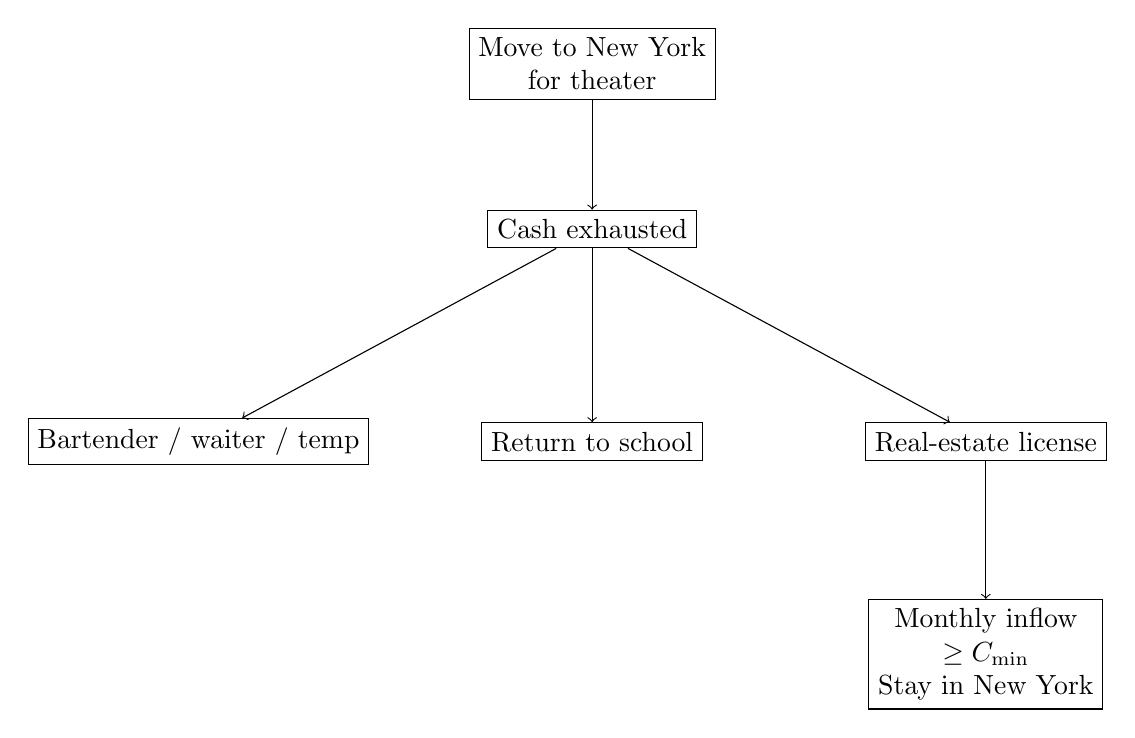
\begin{tikzpicture}[x=1cm,y=1cm]
\node[draw, rectangle, align=center] (start) at (0,0) {Move to New York\\for theater};
\node[draw, rectangle, align=center] (cash) at (0,-2.1) {Cash exhausted};
\node[draw, rectangle, align=center] (bar) at (-5,-4.8) {Bartender / waiter / temp};
\node[draw, rectangle, align=center] (school) at (0,-4.8) {Return to school};
\node[draw, rectangle, align=center] (license) at (5,-4.8) {Real-estate license};
\node[draw, rectangle, align=center] (stay) at (5,-7.5) {Monthly inflow\\\(\ge C_{\min}\)\\Stay in New York};
\draw[->] (start) -- (cash);
\draw[->] (cash) -- (bar);
\draw[->] (cash) -- (school);
\draw[->] (cash) -- (license);
\draw[->] (license) -- (stay);
\end{tikzpicture}
\end{figure}

The speaker adds a final temporal sharpening: he started in real estate on the day Lehman Brothers filed for bankruptcy. The chapter should not smooth that away. It reinforces the lecture's deeper point that entry does not usually occur under clean conditions. Often the path begins precisely when the surrounding system is unstable.

\section{Niches, Endurance, and the Separation of Scale}

The real-estate case continues. Once the floor has been established, the lecture climbs again toward operating doctrine. The first lesson for someone entering real estate in 2024 is ``riches in niches.'' That slogan becomes meaningful only when paired with endurance. People hop from niche to niche, meet resistance, and interpret resistance as a wall. The speaker's correction is that much of what appears terminal is only local friction.

That distinction matters because it restores time to the argument. A niche is not something we merely discover. It is also something we remain inside long enough to exploit.

The lecture then escalates from personal doctrine to market scale. This is where careful notation becomes indispensable, because several enormous numbers are placed side by side, and the risk of confusion is high.

\begin{table}
\centering
\begin{tabular}{|l|l|l|}
\hline
Quantity & Value & Type \\
\hline
Best Wall Street month & \(\$80{,}000\) & Personal monthly income \\
Acai business output & \(> \$20{,}000{,}000\) & Annual business scale \\
Ryan Serhant annual total & \(\$22{,}000{,}000\) & Annual earnings claim \\
Annual real-estate sales & \(\approx \$4.5 \times 10^9\) & Sales volume \\
Mercedes-Benz Miami sellout & \(\approx \$1.4 \times 10^9\) & Project transaction value \\
Largest single home sale & \(\approx \$195 \times 10^6\) & Asset sale value \\
\hline
\end{tabular}
\end{table}

The table does only one thing, but it does it decisively: it prevents us from collapsing income, revenue, project value, and sales volume into one emotional blur called ``money made.'' The lecture is full of spectacle; the notes must keep the objects distinct.

The same interview then turns to billionaires and the value of time. The speaker's point is not that the rich always spend freely or always economize aggressively. The point is that they price the situation correctly. They can be lavish when the use of money makes sense and cheap when it does not. The restaurant anecdote is really an anecdote about time compression. They do not wish to spend attention on low-yield decisions.

The final lesson of the real-estate block is that sales is the great skill of the new economy. That statement is polemical, but its mechanism is straightforward enough: sales converts energy into inflow; diversified inflow enlarges optionality. The lecture then places this against a fading social script of debt, credential, fixed employment, and prepackaged domestic aspiration. Whether we accept that social diagnosis in full is not the issue here. What matters is the structure of the argument: sales is treated as a scalable interface between the individual and opportunity.

The host then performs another recap. He does not merely praise the interview. He extracts a transportable maxim: scared money does not make money. That recap turns the real-estate case from biography into rule and prepares the last shift of register.

\section{Gary Vee and the Economics of Role Fit}

The final interview with Gary Vee changes the style of the lecture. We leave concrete sector mechanics and enter a more temperamental region. The first advice to the younger self is to trust intuitive judgment and to fix the inability to be candid with people one loves in work. The lecture is no longer asking only how wealth grows. It is asking whether the agent is internally aligned enough to bear the chosen role.

This is followed by a sharp account of scaling. Entrepreneurship is described as repeated loss interrupted by occasional win. The lecture's value here lies not in formal probability theory, which it does not provide, but in the refusal of glamour. Lack of patience, entitlement, and the need to appear successful are treated as structural liabilities.

\subsection{Question \& Answer}

\paragraph{Question.} Do we need to be number one?

\paragraph{Answer.} The lecture's answer is no. Gary Vee resolves the tension by distinguishing prestige from payoff and role from title. The example of the number three at Facebook is meant to show that elite operators inside massive systems can out-earn the vast majority of nominal number ones. The force of the claim is rhetorical, but the lesson is exact: role fit dominates vanity.

This answer matters because it retroactively reorganizes the whole chapter. The first finance case emphasized discipline and resource conservation. The acai entrepreneur added opportunity recognition and horizon selection. The real-estate case added survival floors, compounding, specialization, and sales. Gary Vee completes the picture by insisting that none of these techniques can substitute for fit between person and role.

The final beats of the interview make the same point from the opposite side. Many young people are told to listen upward --- to mentors, parents, teachers, public figures. Gary Vee's correction is that advice is only useful if filtered through actual self-knowledge. Again the lecture resists flattening itself into a universal slogan. Even anti-conventional advice must be fitted to the person receiving it.

\section{Summary}

The lecture unfolds as a sequence of increasingly explicit constraints. First, surplus must be protected: leakage destroys accumulation before returns ever matter. Next, horizons must be separated: business-building is long, market positioning is shorter and benchmarked. Then comes the decisive threshold: if monthly inflow does not clear the cash floor, there is no long run in which compounding can operate. Once survival is secured, the lecture turns toward niches, endurance, sales, and the value of time. Finally, it denies that wealth is exhausted by scale or by visible rank. The deepest question is not only how much money can be made, but what kind of life, time horizon, and institutional role a given person can actually carry well.

In that sense the chapter gives us a serious if unconventional model. Wealth is not a single formula. It is the composition of several simpler ones: preserve surplus, survive the floor, allow time to act, specialize, sell, and choose a role that fits the structure of the self.